\section{国内外研究现状及难点}
\label{sec:intro:background}

%本节说了什么
不同应用场景下的时间隐通道构造方法,已经有多种可行方案被提出。
%本节包含的内容
本节主要介绍基于移动互联网的时间隐通道的发展现状,以及时间隐通道在保证鲁棒性方面采取的策略,最后介绍常用的时间隐通道检测方法。

\subsection{基于移动互联网的时间隐通道}
\label{sec:intro:background:ctc}

%在移动互联网环境下,构建时间隐通道,应当遵守怎样的约束
时间隐通道的最基本约束,便是传输过程需要具备隐蔽性,能够抵御中间方的各种检测方法。如图\nref{fig:1:covert-channel},中间方Warden对Alice及Bob的所有数据进行监听,隐蔽信道和宿主信道的所有传输特征均可得到。对于监听者来说,特定时刻观测的传输过程,一定属于隐蔽信道和宿主信道中的一种。根据关于宿主信道传输特征的先验知识,判断当前传输过程是否与先验知识相符,这种检测方式是监听者常用的基本方法。

根据常用的时间隐通道构造方法,可检测的传输特征包括IPD、数据包长度以及数据包发送顺序,符合抗检测性约束的时间隐通道方案,应当以不破坏分布一致性为原则。在移动互联网环境下,受网络噪声干扰及空口传输的不确定性,时间隐通道的受噪声影响产生误码概率较高,时间隐通道在设计中应当考虑检错及纠错能力,保证传输可靠性。

%常用的构建方法
\insertFigure{
	\begin{figure}
		\centering
        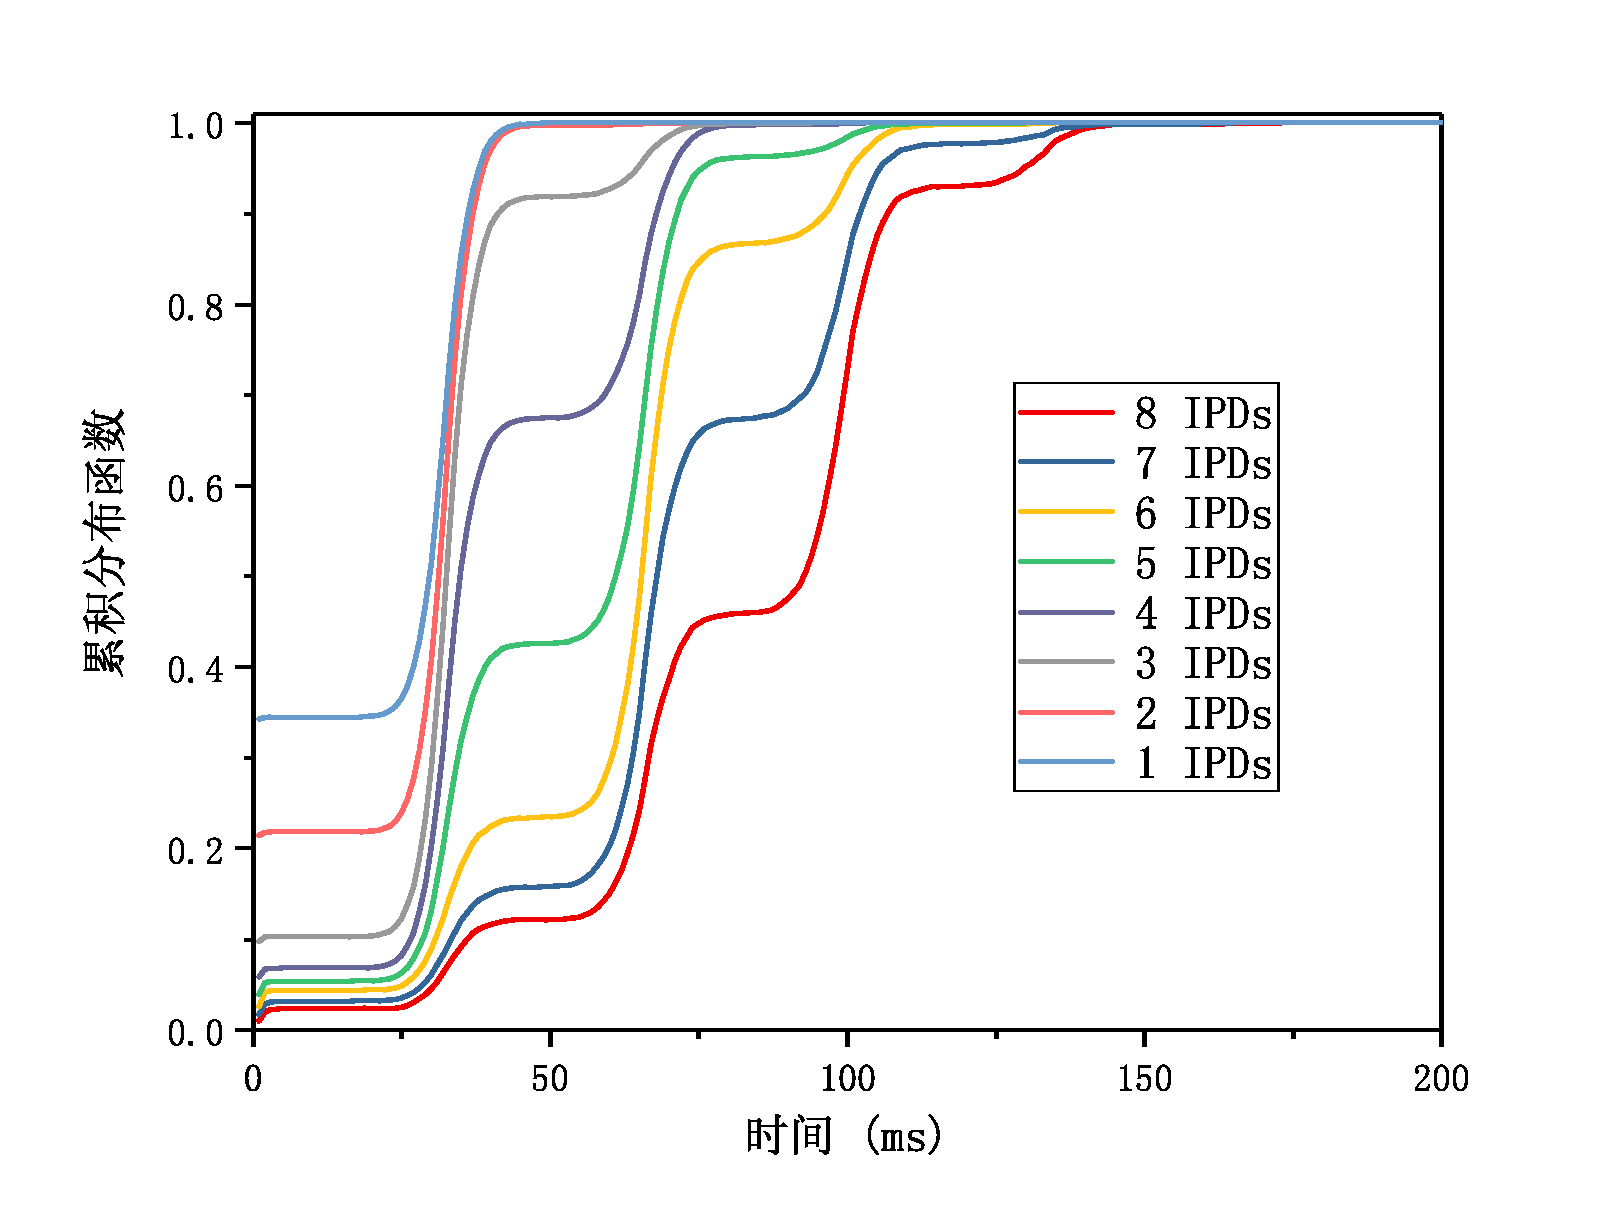
\includegraphics[width=0.75\textwidth]{chapters/chapter1/figures/m-ipds.pdf}
        \caption{VoLTE场景中m-IPDs的累积分布函数}\label{fig:1:m-ipds-cdf}
	\end{figure}
}

移动互联网环境下,已经有一些时间隐通道构建方法,并在测试中具有良好的表现。Skype是一款广泛应用的社交软件,支持基于VoIP的音视频通话功能,在国际市场中占有一定份额。利用Skype通话时具备的端到端传输特征,基于IPD特征构建时间隐通道是可行的。受限于Skype通话质量的约束,数据包的端到端传输延迟必须在100 ms以内,时间隐通道在调制中对IPD的调整具有上限约束;由于音视频通话中的数据量较大,产生的数据包较多,要求时间隐通道调制过程不能阻塞数据包传输,否则导致用户体验及隐通道隐蔽性的损失;另外一点,Skype数据包发送频繁,具有较小的IPD分布,受网络噪声的影响,传输抖动对时间隐通道的鲁棒性具有破坏性,要求时间隐通道方案具备足够的健壮性。\nupcite{7346833}通过改变隐蔽消息与IPD之间的对应关系,将L bit的数据对应到N个数据包,利用一组而不是单个IPD构造传输特征,是解决该问题的一种方法。如图\nref{fig:1:m-ipds-cdf},通过增加统计的IPD数量,CDF统计分布出现离散化,具备了选值的基础条件,同时提高了鲁棒性。

\insertTable{
	\begin{table}[]
        \centering
        \caption{常见VoIP应用的数据包发送速率}
        \label{tab:1:voip-packet-speed}
        \begin{tabular*}{0.4\textwidth}{@{\extracolsep{\fill}}cc}
        \toprule
        应用类型 & 数据包发送速率 \\ 
        \midrule
        微信 & 125 packets/s \\ 
        QQ & 157$\sim$189 packets/s \\
        Skype & 150 packets/s \\
        \bottomrule
        \end{tabular*}
    \end{table}
}

除了通过IPD进行调制,利用数据包长度构建时间隐通道也是可行的。\nupcite{LIANG2018144}借助VoIP的数据包数量多的优势,在合理添加校验信息的基础上,具备更好的性能表现。VoIP中的数据包类型一般分为语音数据包及视频数据包,综合数据包发送速率如表\nref{tab:1:voip-packet-speed}\nupcite{LIANG2018144,LIANG2018162},随着视频分辨率及编码方式的变化,数据包发送速率对应变化。基于数据包长度的时间隐通道,需要在发送方设定一个发送缓冲区,首先将待发送的数据包加入缓冲区,根据待发送数据的需求,调整缓冲区中的数据包顺序,最后执行发送操作。为降低误码率,通常需要结合前向纠错编码或检错码,对网络噪声中丢包或乱序产生的干扰进行消除。

另一方面,YouSkyde利用Skype视频通话中的随机丢包事件,构造出了高性能的存储隐通道。在Skype视频通话中,产生的丢包事件与数据包长度及发送密度均无相关关系,并且在不同的丢包率状态下,skype会自动对部分数据进行重传。通过对重传阶段的数据进行替换,利用原始信道的重传行为,实现隐蔽数据的传输,在传输模式及传输特征方面均符合宿主信道的特征。由于对重传的视频数据进行了替换,视频通话质量存在损失,通过结合实际通话需求及原始视频质量分布,构建隐通道产生的视频质量损失,相较网络噪声的影响,并不是主要因素。\nupcite{mazurczyk2016youskyde}

%各种方法的总结,以及为何不能应用在VoLTE环境中
移动互联网环境下的时间隐通道,多数延续了以太网下时间隐通道的构建方法,更多的聚焦在如何均衡鲁棒性及传输性能。面对新的网络及应用环境,提供了不同的时间隐通道构造场景,应该有针对性的构造方法与之对应。本文在研究了VoLTE环境下视频数据包的丢包特征后,提出了基于主动丢包的时间隐通道构造方式,充分挖掘了这一场景下的应用潜力。

\subsection{时间隐通道的鲁棒性策略}
\label{sec:intro:background:robustness}

%首先说明,时间隐通道因为自身的特性,在传输可靠性上,不如Overt Traffic
时间隐通道本质上是附加在宿主信道的寄生信道,相对于宿主信道,具有较低的信噪比,重传确认及差错控制效率较低。为提高时间隐通道的可用性,较低的误码率,类似检错码、纠错码及卷积码等编码方式被应用在信道编码过程中,利用编码中的冗余信息,对噪声产生的跳变及数据丢失进行检验和纠正。

%现有的时间隐通道方案,在保证鲁棒性反面,采用了怎样的手段,比如添加检错信息、重传、纠错编码等
在信道编码过程采用可靠性编码,是提高传输可靠性的常用方法。格雷码是一种与奇偶校验码具有同等校验能力的编码,相邻的数据的二进制编码只有一个比特位发生改变。这种编码特征,在易发生比特跳变的场景,具有一定的可靠性保证。例如在VoIP通话中,RTCP(Real-time Transport Control Protocol)数据包之间会间隔RTP数据包,通过调整RTCP间隔数据包的数量,实现具有良好抗检测性的时间隐通道。\nupcite{ZHANG201866}但网络丢包和乱序是不可避免的,接收方观测到的RTCP数据包间隔的RTP数据包数量,会出现随机波动。通常噪声导致的波动在一个数量级以内,格雷码的应用,有效降低了误码位数,保证大部分数据的正确性。

喷泉码是抹除码的一种,类似喷泉由下而上的喷涌过程,不断传输有效数据信息,接收到足够符号之后,接收方根据已知数据完整恢复消息内容。喷泉码的应用场景,是传输信道的接收方只有成功或失败两种结果,出现传输错误的数据块不进行处理。喷泉码的编码过程,需要结合特定的编码矩阵,利用矩阵中的对应关系,完成原始符号与编码符号的线性映射。接收方每次接收到的符号,都是多个原始符号的组合结果,通过喷泉码解码器,逐步还原所有的原始符号。\nupcite{6296078}

\insertFigure{
	\begin{figure}
		\centering
        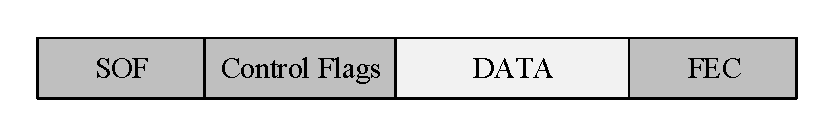
\includegraphics[width=0.75\textwidth]{chapters/chapter1/figures/frame-struct.pdf}
        \caption{常用的数据帧格式}\label{fig:1:frame-struct}
	\end{figure}
}

传输内容的结构化,也是时间隐通道中保证鲁棒性的常用方法。如图\nref{fig:1:frame-struct},参照IP数据包的数据帧格式,结构化数据一般包括起始标志SOF(Start of Frame)、负载数据DATA、辅助标记Flags及校验信息几个部分。这种数据帧划分方式,有效保证了数据完整性,在添加FEC(Forward Error Correction)后,能够纠正一定范围内的传输错误。\nupcite{LIANG2018144}

%这些方法,对应用场景的限制及不足
在VoLTE通话场景中,基于主动丢包方式构造时间隐通道,需要对数据包传输序号进行监测,对鲁棒性影响最大的是噪声中的丢包事件。为保证较好的抗检测性,主动丢弃的数据包数量要远少于网络噪声产生的丢包,导致信噪比极低。以上鲁棒性方法的前提,是接收数据中的大多数均为正确数据,只有少量的错误需要进行纠正。而通过主动丢方式构建的时间隐通道,在解调过程中,需要由众多噪声中进行分辨,简单的鲁棒性策略无法实现该目标,需要多层多维度的去噪方法。

\subsection{时间隐通道的检测方法}
\label{sec:intro:background:detect}

%检测时间隐通道,通常从哪几个要素方面进行考虑
不同于存储隐通道,时间隐通道的构建对数据本身不产生影响,存储隐通道检测方法中使用的数据匹配核查,对时间隐通道是无效的。根据时间隐通道的构建方法,数据包传输特征中的顺序及发送间隔,是出现异常特征的两个重要方面,现有的检测方法也主要对其进行判别。为有效判别时间隐通道,前期工作中需要对标准状态下的传输特征进行分析,将分析结果作为标准参照,后续的判别工作均基于标准参照进行识别。

%检测判断,主要根据哪些因素来考量,包括分布、一致性
\subsubsection{基于分布曲线的检测}
基于分布曲线的检测方法,需要首先获取样本的IPD分布特征,并计算出CDF曲线。通过对比参照曲线和样本曲线,判断曲线的偏离度,决定样本与标准参照是否为相同分布。在比较方式上,对比曲线的基本趋势,或者通过量化评估方式计算最大偏离度。\nupcite{Cabuk:2004:ICT:1030083.1030108}Kolmogorov-Smirnov测试中判断分布$F(x)$及$G(x)$差异的方式,需要统计$F(x)$及$G(x)$在相同$x$下差值绝对值的下届,并用下届值代表样本与参照之间的差异。除了K-S测试之外,Welch’s t-test也是进行分布差异判别的常用方法。

\insertEquation{
    \begin{equation}
    \label{equ:1:entropy}
		H(X)=-\sum_{x=i}p(x) \cdot \log(p(x))
    \end{equation}
}

\subsubsection{基于熵的检测}
在信息论中,熵代表了每条消息蕴含信息的高低,在时间隐通道检测中,熵代表了统计对象的离散程度。对于参照分布和验本分布来说,通过公式(\nref{equ:1:entropy})计算基于信息学的熵值,或者计算Kullback-Leibler条件熵。\nupcite{Gianvecchio:2007:DCT:1315245.1315284}与基于分布曲线计算方式不同,信息学熵值及Kullback-Leibler条件熵的计算对象为PDF(Probability Density Function),也就是概率密度函数,对应相同$x$时的概率$f(x)$及$g(x)$。通过判断熵值的大小,判定分布一致性,在时间隐通道检测中被证明是有效可行的。\nupcite{5590253}

%在该场景中,主要通过丢包的方法构建时间隐通道,所有,在现有的常用检测方法的基础上,还要对丢包的特征进行分析
\subsubsection{基于主动丢包的时间隐通道检测方法}
传统的时间隐通道检测方法,聚焦于IPD分布的一致性检测,对传输过程中的丢包特征不予判别。现有的检测方法,无法充分证明基于主动丢包的时间隐通道具有足够的隐蔽性。针对VoLTE场景下的丢包特征,需要进行针对性分析,并建立有效的判别规则和检测方法。
